
\documentclass{beamer}
\usepackage[latin1]{inputenc}
\usepackage{wrapfig}

\definecolor{OliveGreen}{cmyk}{0.64,0,0.95,0.40}
\definecolor{MyGrey}{cmyk}{0.2,0.2,0.2,0.5}
%\usecolortheme[named=MyGrey]{structure}
%\usecolortheme[named=OliveGreen]{structure}
\usetheme{CambridgeUS}
%\usecolortheme{CambridgeUS}
%\usetheme{Boadilla}
\newcommand{\ggr}{\color{red}}
\newcommand{\reportauthor}{
Thayabaran~Kathiresan\\
R\' emi~Domingues\\
Agnes Martine~Nielsen\\
Tobias~Wiens}

%\pgfpagesuselayout{4 on 1}[a4paper,border shrink = 5mm, landscape]
\beamertemplatenavigationsymbolsempty % removes pdf-content, for printing


%\setbeamercolor{block}{fg=Red}
%\setbeamercolor{block}{bg=gray}
\setbeamercolor{math text}{fg=OliveGreen}


\subtitle[Machine Learning]{Machine Learning, Advanced Course}
\title{Project: Kernel Principal Component Analysis}
\author{\reportauthor}
\institute{KTH Royal Institute of Technology}



\begin{document}

%%%%%%%%%%%%%%%%%%%%%%%%%%%
\begin{frame}
 \maketitle
\end{frame}
%%%%%%%%%%%%%%%%%%%%%%%%%%%

%%%%%%%%%%%%%%%%%%%%%%%%%%%
\begin{frame}
 \tableofcontents
\end{frame}
%%%%%%%%%%%%%%%%%%%%%%%%%%%



%%%%%%%%%%%%%%%%%%%%%%%%%%%%%%%%%%%%%%%%%%%%%%%%%%%%%%%%%%%%%%%%%%%%%%%%%%%%%%%%%%%%%%%%%%%%%%%%
%%%%%%%%%%%%%%%%%%%%%%%%%%%%%%%%%%%%%%%%%%%%%%%%%%%%%%%%%%%%%%%%%%%%%%%%%%%%%%%%%%%%%%%%%%%%%%%%
% INTRO PCA CONCEPTS

\section[Introduction]{Introduction} % Sectio
%\begin{frame}
%    \frametitle{Principal Component Analysis} % Slide title%
%	\textbf{Purpose}
%	\begin{itemize}
%		\item Principal component space of lower dimension than the initial space
%	\end{itemize}
%
%	\textbf{Steps}
%	\begin{itemize}
%		\item Build the covariance matrix $\bar{C}$
%		\item Calculate the \textit{N} eigenvectors corresponding to the highest eigenvalues obtained by diagonalization of $\bar{C}$
%		\item The representation of X in the principal component space is $Y = PX$, with the rows of P composed of the \textit{eigenvectors} maximizing the variance
%	\end{itemize}
%\end{frame}

\begin{frame}
    \frametitle{Kernel Principal Component Analysis: Motivation} % Slide title
	Take non-linearities into account\\
	\vspace{0.5cm}
	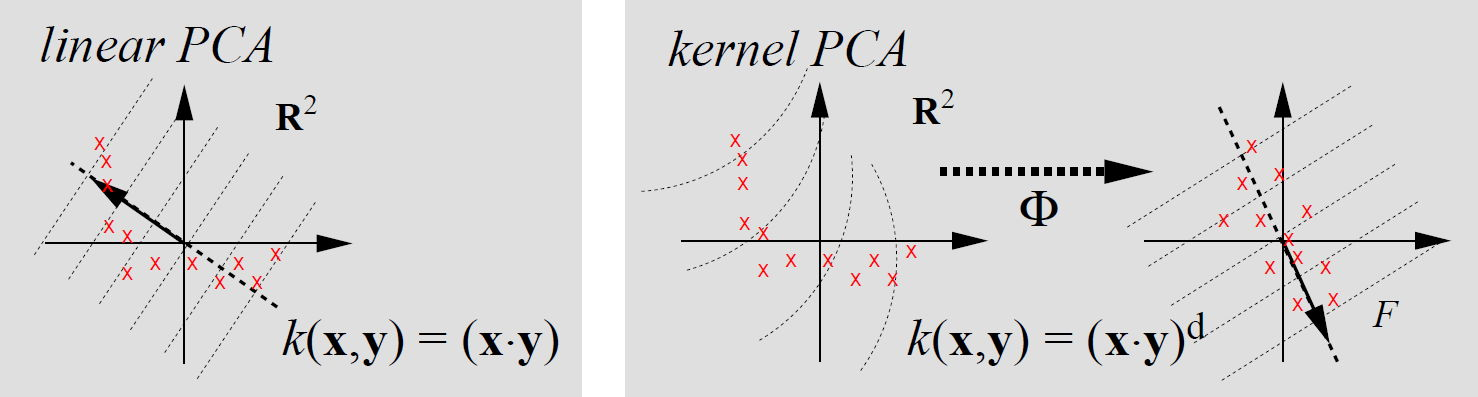
\includegraphics[width=0.8\textwidth]{build/kernel_pca.jpg}    
	
		\begin{itemize}
		\item \textit{PC} are extracted from the high-dimension feature space F
		\item Kernel functions gives us $\Phi(\textbf{x}) \cdot \Phi(\textbf{y})$ for a low computation cost
	\end{itemize}
   
\end{frame}

%    
%	\begin{itemize}
%		\item \textit{PC} are extracted from the high-dimension feature space F which 
%		\item  $\Phi : \mathbb{R}^N \rightarrow F, \textbf{x} \rightarrow \textbf{X}$
%		\item Kernel functions gives us $\Phi(\textbf{x}) \cdot \Phi(\textbf{y})$ for a low computation cost
%	\end{itemize}


% THEORY: KERNEL PCA SLIDES
\section[Theory]{Kernel PCA} % Section
\begin{frame}
  \frametitle{Kernel PCA} % Slide title
    High-dimension feature space F
    \begin{equation} \label{eq:space_definition}
        \Phi : \mathbb{R}^N \rightarrow F, \textbf{x} \rightarrow \textbf{X}
    \end{equation}

    Covariance matrix in F
    \begin{equation} \label{eq:cov_matrix}
        \bar{C} = \frac{1}{l} \sum\limits_{j=1}^{l} \Phi(\textbf{x}_j) \Phi(\textbf{x}_j)^T
    \end{equation}
    
    Assumption: data in F is centered in 0
\end{frame}

\begin{frame}
  \frametitle{Kernel PCA} % Slide title
    Finding eigenvalues and eigenvectors: $\lambda\textbf{V}=\bar{C}\textbf{V}$
    
    Write eigenvectors as follows since $\textbf{V}\in \text{span}\{ \Phi(\textbf{x}_1),\dots,\Phi(\textbf{x}_l)\} $
    \begin{equation} 
\textbf{V} = \sum\limits_{i=1}^{l} \alpha_i \Phi(\textbf{x}_i)
    \end{equation}    
    

   This leads to the problem following eigenvalue problem
   
       \begin{equation} \label{eq:solution}
        l \lambda \boldsymbol{\alpha} = \textbf{K} \boldsymbol{\alpha}
    \end{equation}
    
    with
    
    \begin{equation} \label{eq:k_matrix}
        K_{ij} := (\Phi(\textbf{x}_i) \cdot \Phi(\textbf{x}_j))
    \end{equation}

\end{frame}

\begin{frame}
  \frametitle{Kernel PCA} % Slide title

    Principal components of a data point $\Phi(\textbf{x})$
    \begin{equation} \label{eq:components_extraction}
        (\textbf{V}^k \cdot \Phi(x)) =  \sum\limits_{i=1}^{l} \alpha_i^k (\Phi(\textbf{x}_i) \cdot \Phi(\textbf{x}))
    \end{equation}
    
We replace all inner products in F with a kernel function. We use polynomial kernel in our experiments,

$$
k(x,y) = (x\cdot y)^d
$$    
    
\end{frame}

\section[Results]{Results} % Section
\begin{frame}
    \frametitle{Experiment} % Slide title
        \begin{wrapfigure}{r}{0.4\textwidth}
  \begin{center}
    \includegraphics[width=0.35\textwidth]{build/usps.png}
  \end{center}
\end{wrapfigure}
    For testing the performance of the Kernel PCA, we have chosen the digits classification problem. We used the USPS (US Postal Service) Handwritten digits. This data set contains 9300 examples, for better simulation we have used\\

    \vspace{0.5cm}
    \textbf{Training Data} : 3000\\
    \textbf{Test Data}   : 2000 \\

\vspace{0.5cm}
\textbf{Types of Classifier used:}\\
Multivariate Gaussian (Linear Classifier)\\
Linear Support Vector Machine
\end{frame}

\begin{frame}
\frametitle{The articles results}
Classification using separating hyperplane (SVM)\\
\vspace{0.5cm}
In case of linear PCA ($d=1$) best result is 8.6\% error for PC$=128$.\\
Non-linear PCA ($d=2,\dots,6$ and PC$=128$) gives around 6\% error\\
With $d>2$ and 2048 components gives around 4\% error\\
\end{frame}

\begin{frame}
\frametitle{Our results}

\begin{figure}
\centering
\caption{Classification using Gaussian Multivariate Classifier}
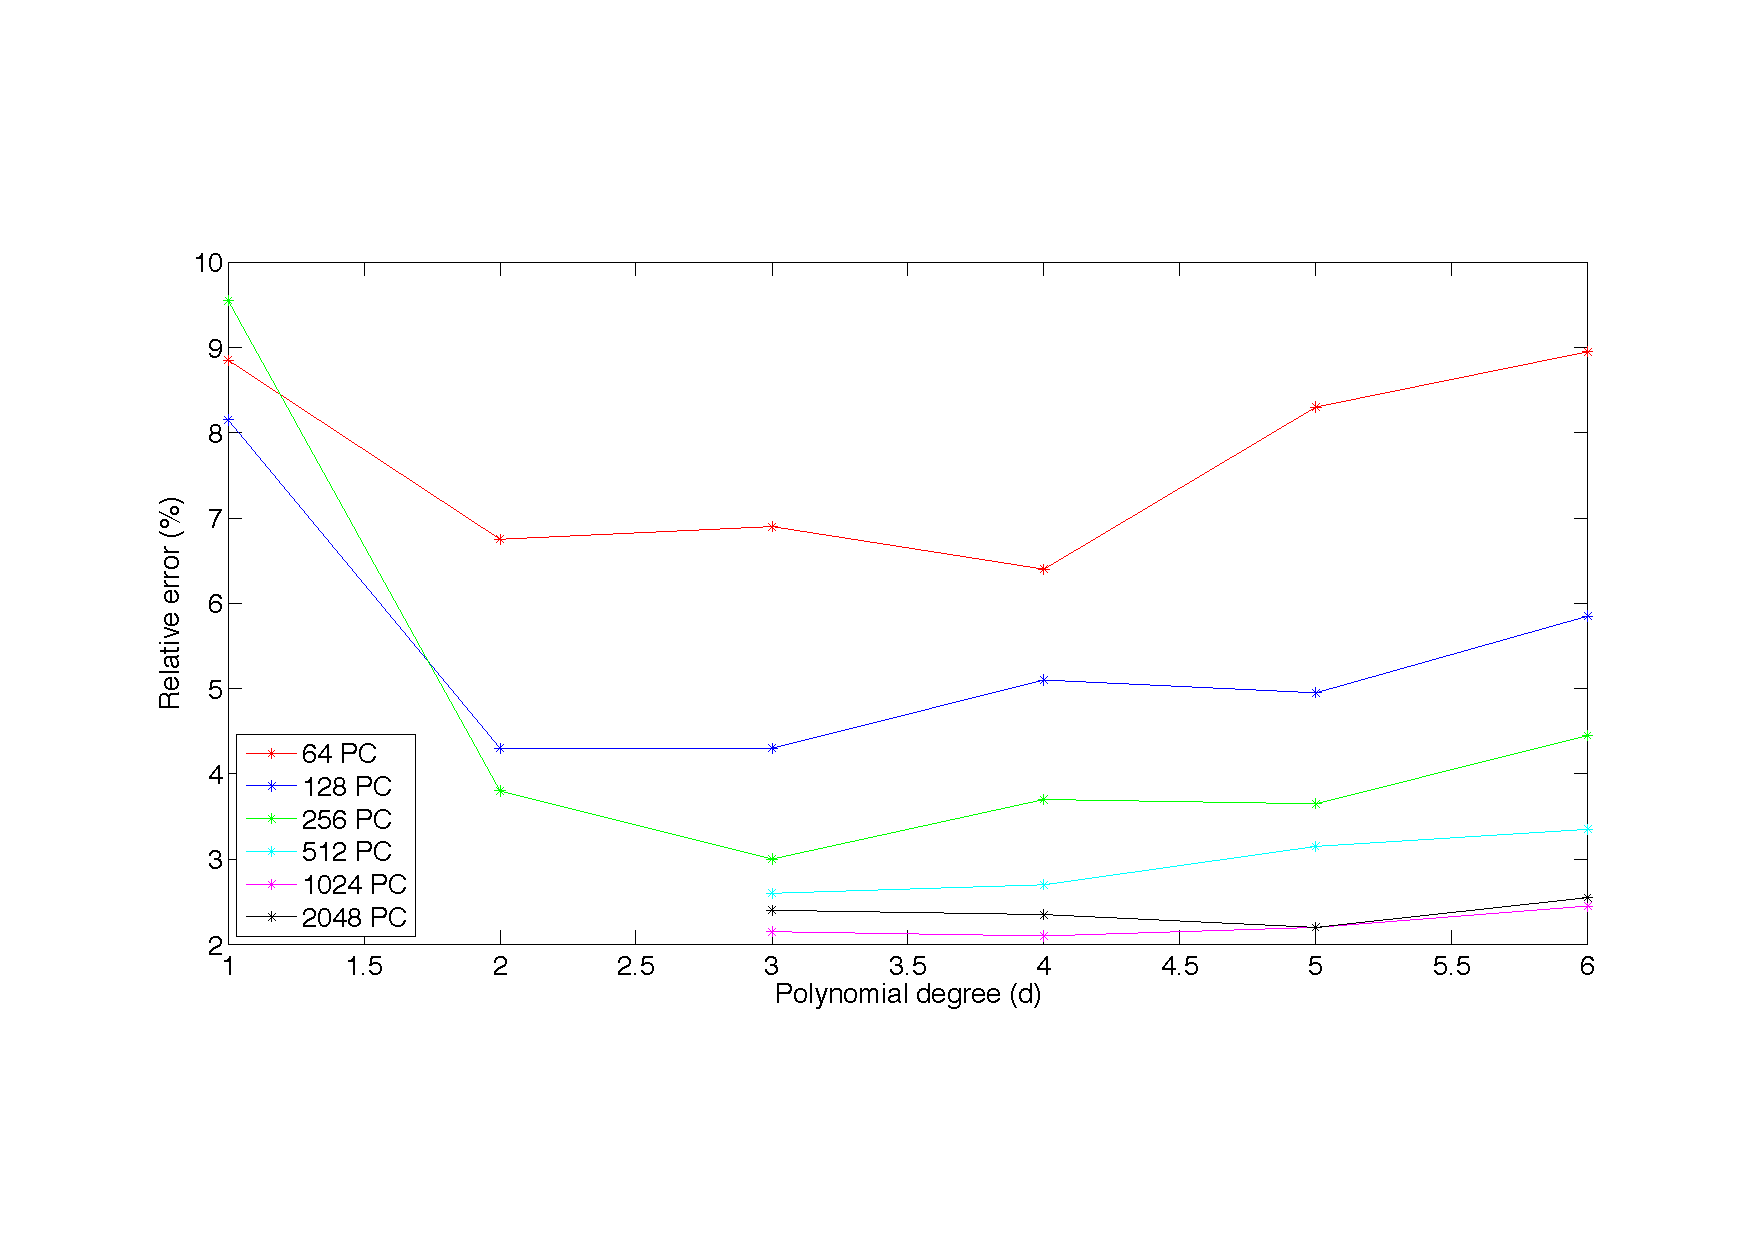
\includegraphics[width=0.9\textwidth]{build/errorplotGMMclass.pdf}
\end{figure}

Matlab command: \texttt{classify}
\end{frame}

\begin{frame}
\frametitle{Our results}

\begin{figure}
\centering
\caption{Classification using SVM}
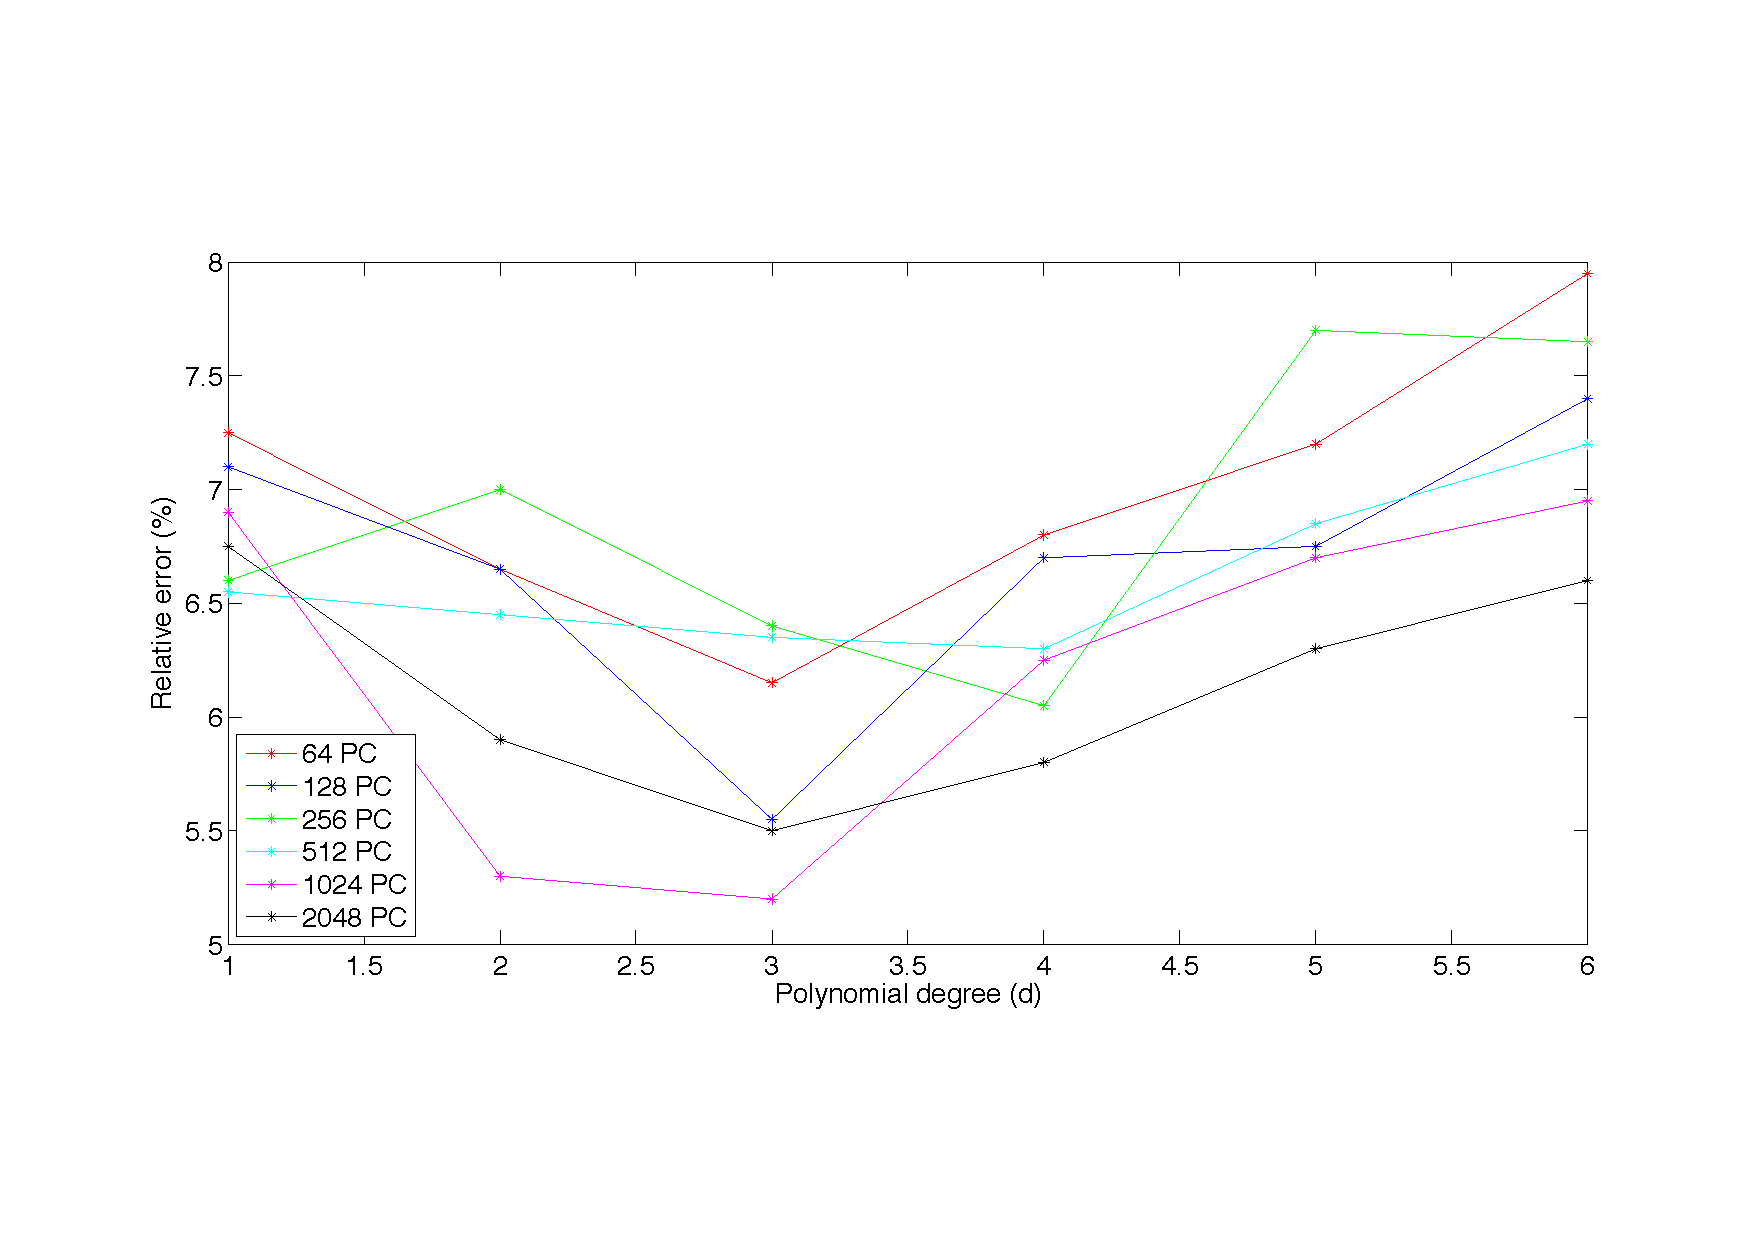
\includegraphics[width=0.9\textwidth]{build/errorplotSVMclass.pdf}
\end{figure}

Matlab command: \texttt{svmtrain} (using LIBSVM)
\end{frame}

%DISCUSSION

\section[Discussion]{Discussion} % Section

\begin{frame}
    \frametitle{Discussion} % Slide title
	\textbf{Advantages}
	\begin{itemize}
		\item Better results with linear classifiers: Kernel PCA extends PCA by extracting non-linear principal components allowing better performances for linear classifications
		\item Those components are computed by only solving the eigenvalue problem, which is done in a low complexity due to the Kernel methods
	\end{itemize}

	\textbf{Suggested improvements}
	\begin{itemize}
		\item Adapt Kernel PCA to current PCA methods suitable for huge datasets
		\item Scaling factor applied to $\bar{C}$ is \textit{l}, should be $l-1$ to remove the bias (Bessel's correction)
	\end{itemize}
\end{frame}



\begin{frame}
\frametitle{Questions?}
\begin{center}
\huge{Questions?}
\end{center}
\end{frame}


\begin{frame}
Equivalent system to $\lambda\textbf{V}=\bar{C}\textbf{V}$

    \begin{equation} \label{eq:eq_system}
        \lambda (\Phi(\textbf{x}_k) \cdot \textbf{V}) = (\Phi(\textbf{x}_k)) \cdot \bar{C} \textbf{V})\text{ for }k = 1,...,l~with~\textbf{V} = \sum\limits_{i=1}^{l} \alpha_i \Phi(\textbf{x}_i)
    \end{equation}

\end{frame}

\end{document}